\documentclass[tikz,border=10pt]{standalone}
\usepackage{tikz}

\begin{document}
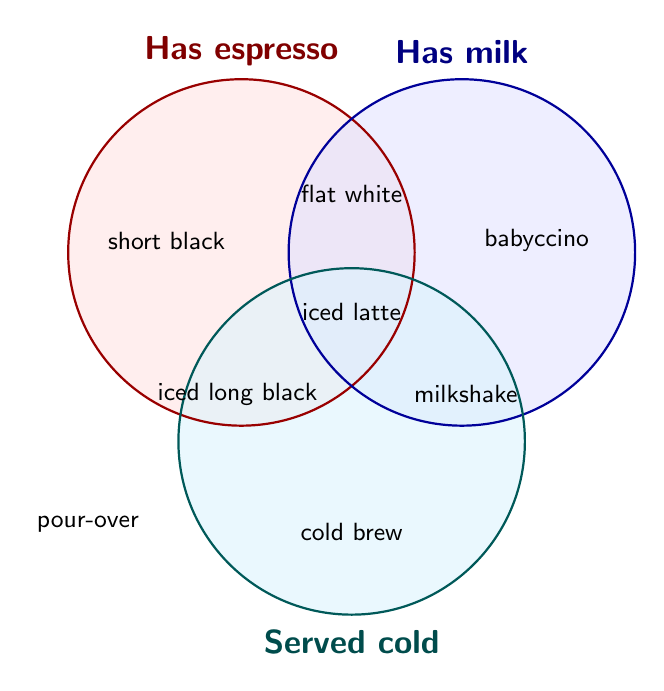
\begin{tikzpicture}[
  every node/.style={font=\sffamily},
  drink/.style={font=\sffamily\small, align=center},
  setname/.style={font=\sffamily\bfseries\large}
]

% ---- circles (E = espresso, M = milk, C = cold) ----
\begin{scope}
  \fill[red!12, fill opacity=0.55] (-1.4,1.0) circle (2.2);
  \fill[blue!12, fill opacity=0.55] (1.4,1.0) circle (2.2);
  \fill[cyan!15, fill opacity=0.55] (0,-1.4) circle (2.2);
\end{scope}
\draw[thick, red!60!black]  (-1.4,1.0) circle (2.2);
\draw[thick, blue!60!black] ( 1.4,1.0) circle (2.2);
\draw[thick, teal!70!black] ( 0,-1.4) circle (2.2);

% ---- set names ----
\node[setname, red!50!black]  at (-1.4, 3.55)  {Has espresso};
\node[setname, blue!50!black] at ( 1.4, 3.55)  {Has milk};
\node[setname, teal!60!black] at ( 0,  -3.95)  {Served cold};

% ---- drinks in their regions ----
% espresso only
\node[drink] at (-2.35, 1.15) {short black};
% milk only
\node[drink] at ( 2.35, 1.15) {babyccino};
% cold only
\node[drink] at ( 0.00,-2.55) {cold brew};
% espresso + milk (hot)
\node[drink] at ( 0.00, 1.75) {flat white};
% espresso + cold (no milk)
\node[drink] at (-1.45,-0.80) {iced long black};
% milk + cold (no espresso)
\node[drink] at ( 1.45,-0.80) {milkshake};
% all three
\node[drink] at ( 0.00, 0.25) {iced latte};
% outside all three
\node[drink] at (-3.35,-2.45) {pour-over};

\end{tikzpicture}
\end{document}